\section[Composite Model Results]{Composite Model Results}

\begin{frame}{Current Status \& Key Results}
\begin{columns}
\begin{column}{0.5\textwidth}
\textbf{Completed:}
\begin{itemize}
    \item \textbf{All 5 models} successfully trained (200 epochs each)
    \item \textbf{Comprehensive evaluation} across 4 dataset types
    \item \textbf{Architecture debugging} completed (Experiment 192)
    \item \textbf{Performance analysis} with statistical metrics
\end{itemize}
\end{column}
\begin{column}{0.5\textwidth}
\textbf{Key Findings:}
\begin{itemize}
    \item \textbf{Default LodeSTAR} architecture performs best
    \item \textbf{Moderate performance} on different shapes
    \item \textbf{Optimized parameters} identified
\end{itemize}
\end{column}
\end{columns}
\end{frame}

\begin{frame}{Composite Model Results}
\begin{center}
\begin{tabular}{|c|c|c|c|}
\hline
\textbf{Dataset Type} & \textbf{F1 Score} & \textbf{Precision} & \textbf{Recall} \\
\hline
Same Shape, Same Size & \textbf{0.808} & \textbf{0.862} & \textbf{0.781} \\
\hline
Same Shape, Diff Size & \textbf{0.241} & \textbf{0.713} & \textbf{0.161} \\
\hline
Diff Shape, Same Size & \textbf{0.675} & \textbf{0.850} & \textbf{0.605} \\
\hline
Diff Shape, Diff Size & \textbf{0.143} & \textbf{0.739} & \textbf{0.103} \\
\hline
\end{tabular}
\end{center}

\textbf{Composite Analysis:}
\begin{itemize}
    \item \textbf{High Precision}: Consistently high (>0.7) across all datasets, indicating trustworthy detections.
    \item \textbf{Size Sensitivity}: Recall drops significantly on "Different Size" datasets.
    \item \textbf{Shape Discrimination}: Performs well on "Diff Shape, Same Size", proving the ensemble can classify effectively.
\end{itemize}
\end{frame}

\begin{frame}{Composite Model Results}
    \begin{figure}
        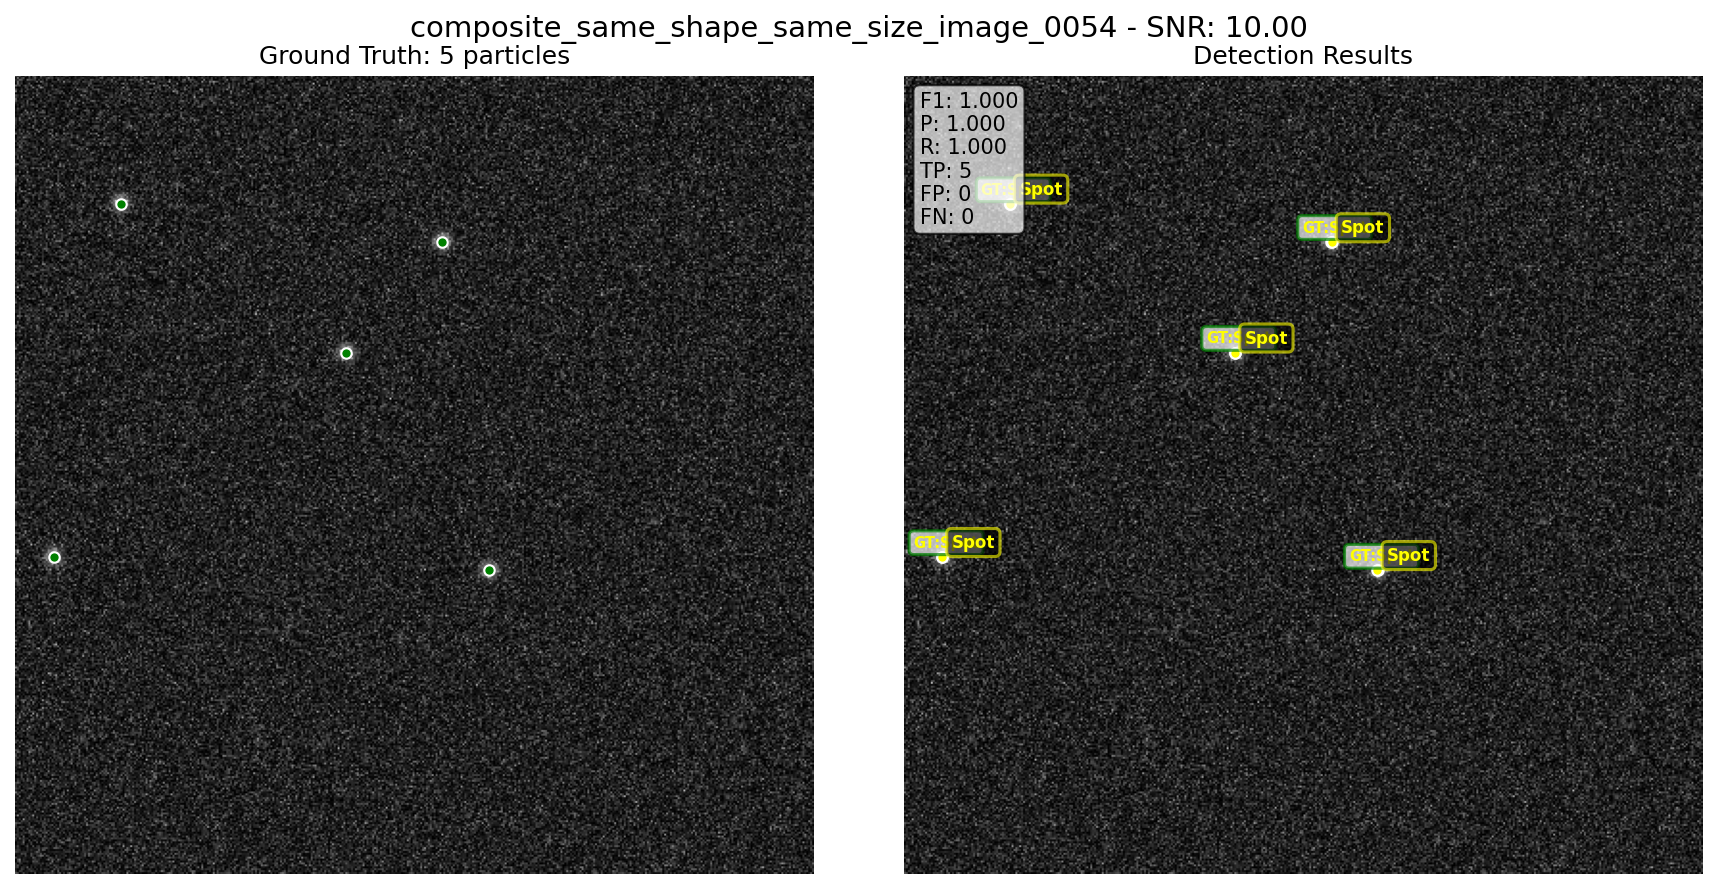
\includegraphics[width=\textwidth]{imglib/Results/composite_same_shape_same_size_image_0054.png}
    \end{figure}
\end{frame}

\begin{frame}{Composite Model Results}
    \begin{figure}
        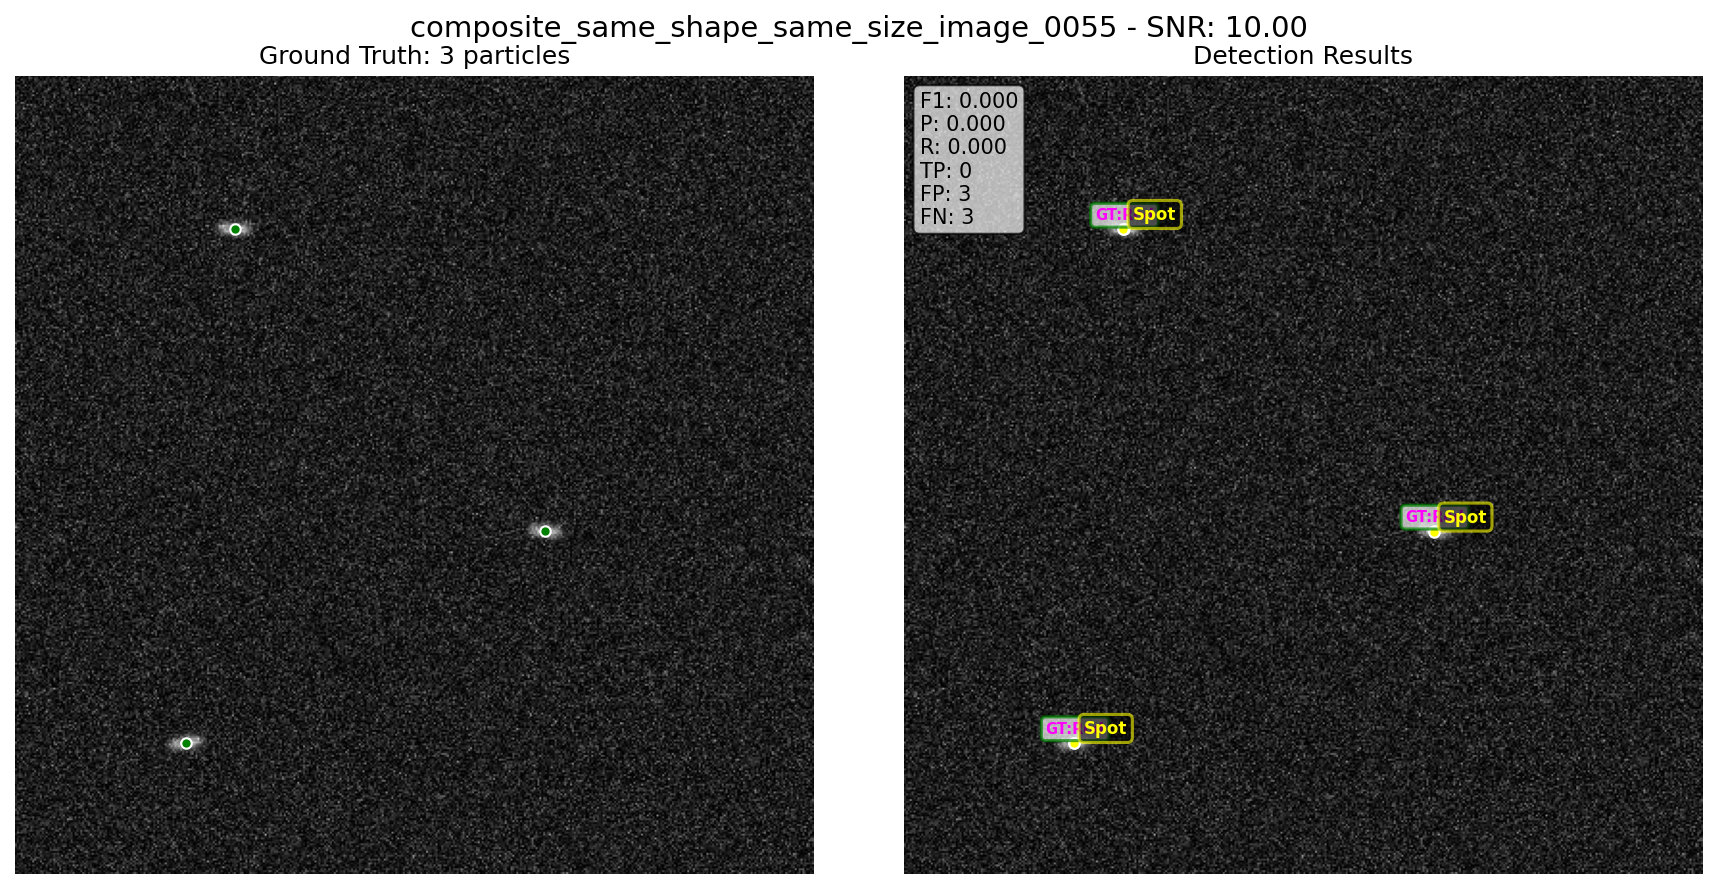
\includegraphics[width=\textwidth]{imglib/Results/composite_same_shape_same_size_image_0055.png}
    \end{figure}
\end{frame}

\begin{frame}{Composite Model Results}
    \begin{figure}
        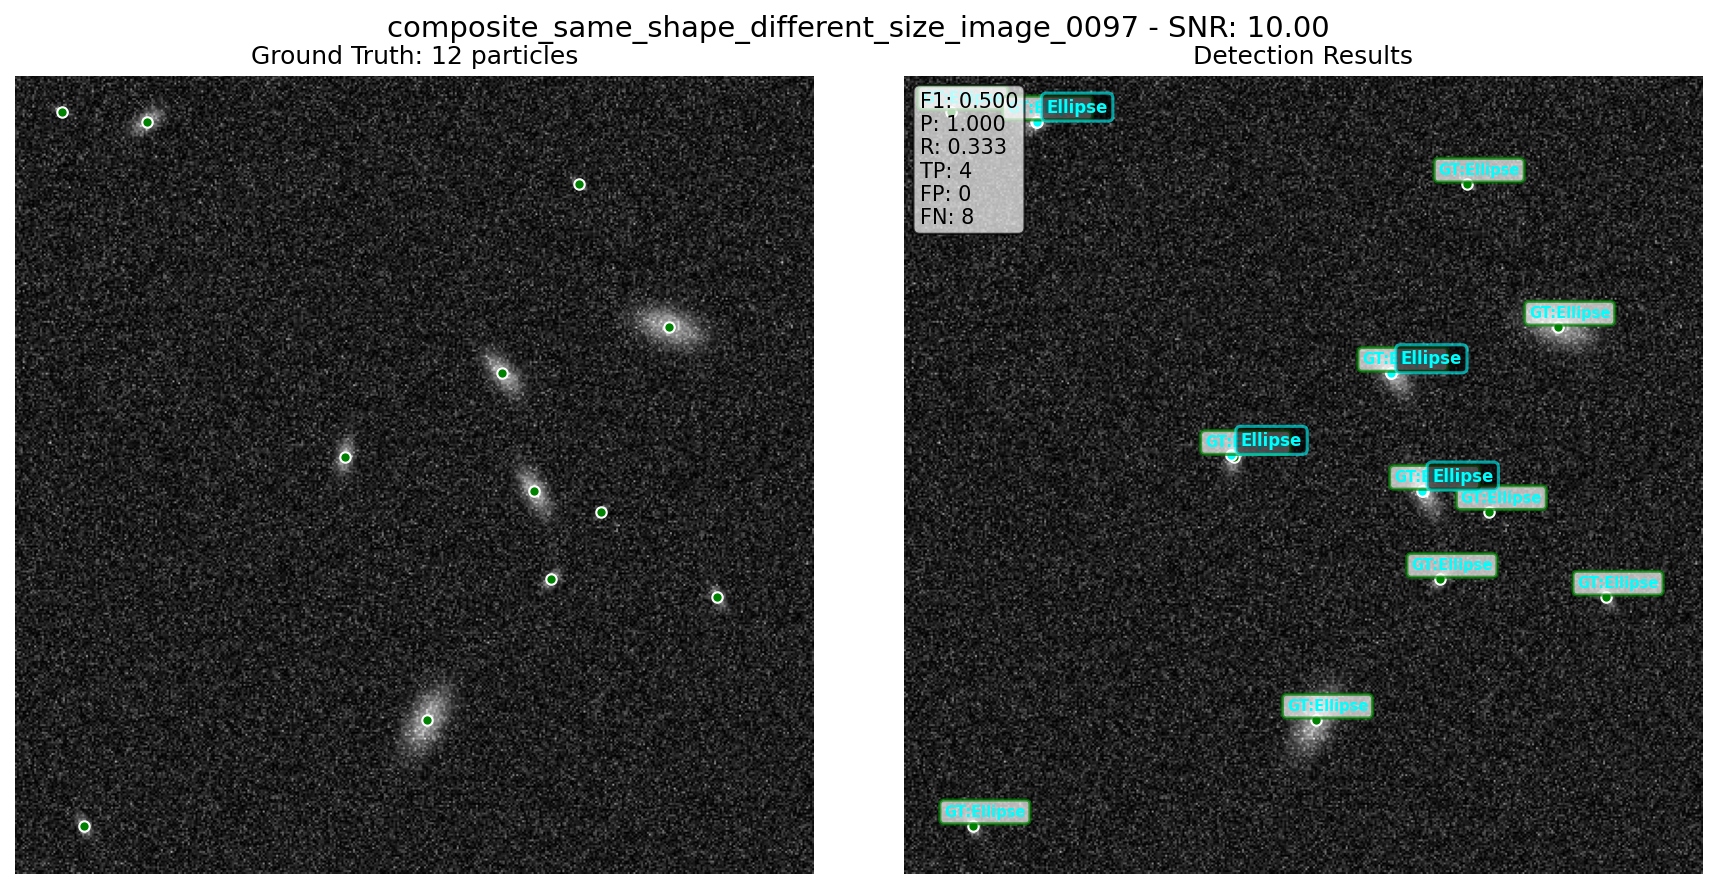
\includegraphics[width=\textwidth]{imglib/Results/composite_same_shape_different_size_image_0097.png}
    \end{figure}
\end{frame}

\begin{frame}{Composite Model Results}
    \begin{figure}
        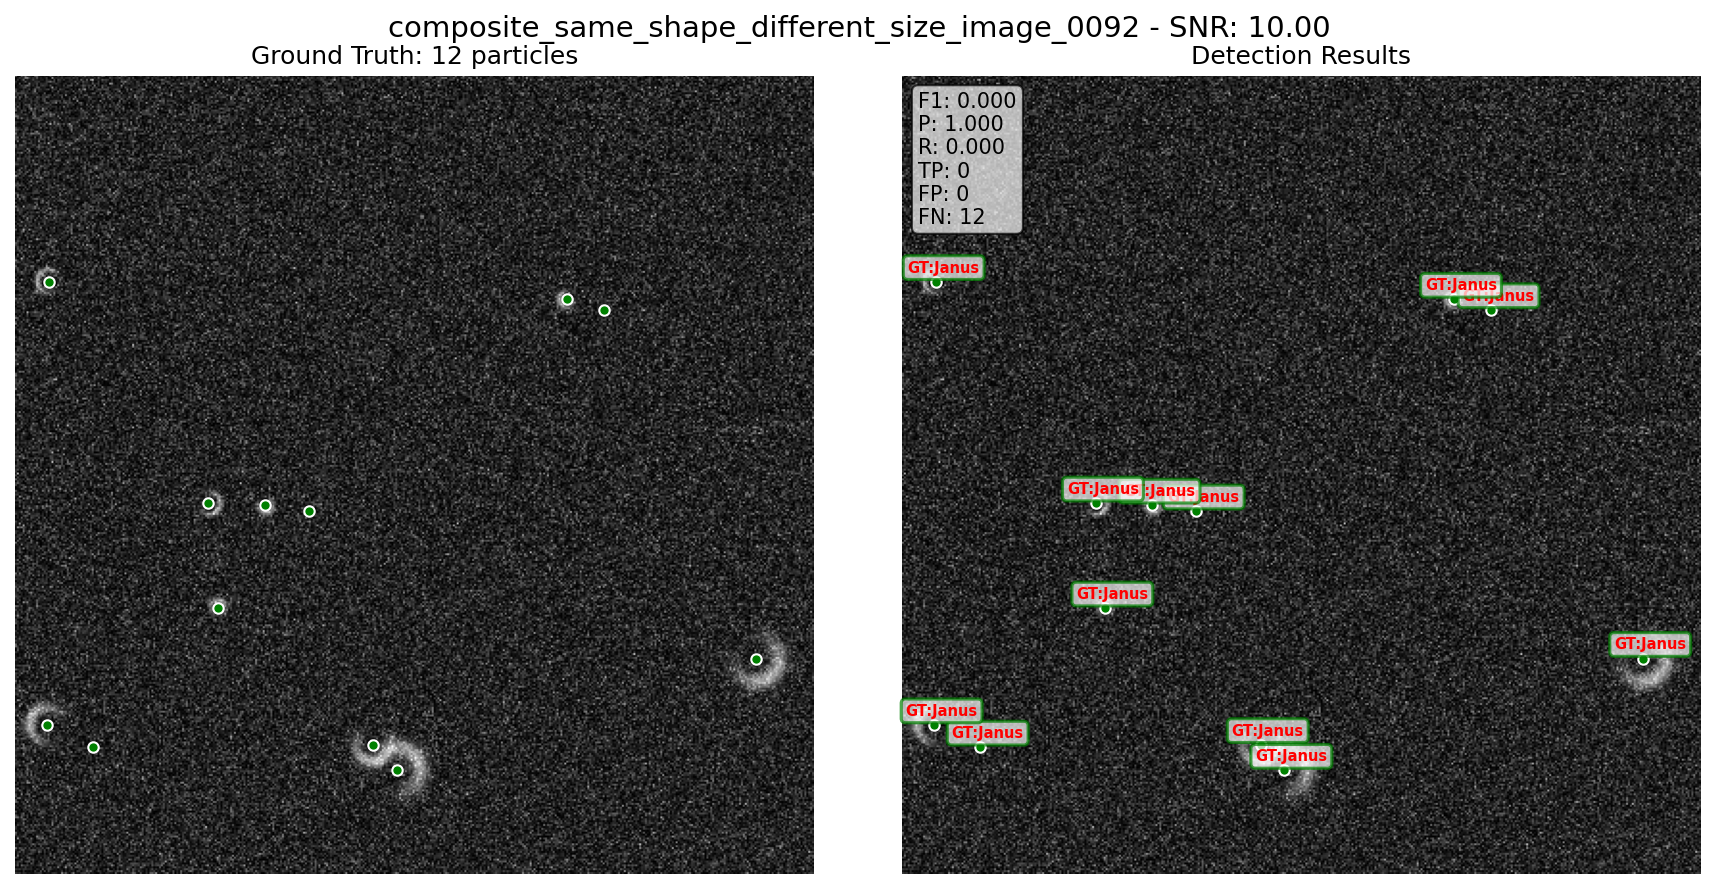
\includegraphics[width=\textwidth]{imglib/Results/composite_same_shape_different_size_image_0092.png}
    \end{figure}
\end{frame}

\begin{frame}{Composite Model Results}
    \begin{figure}
        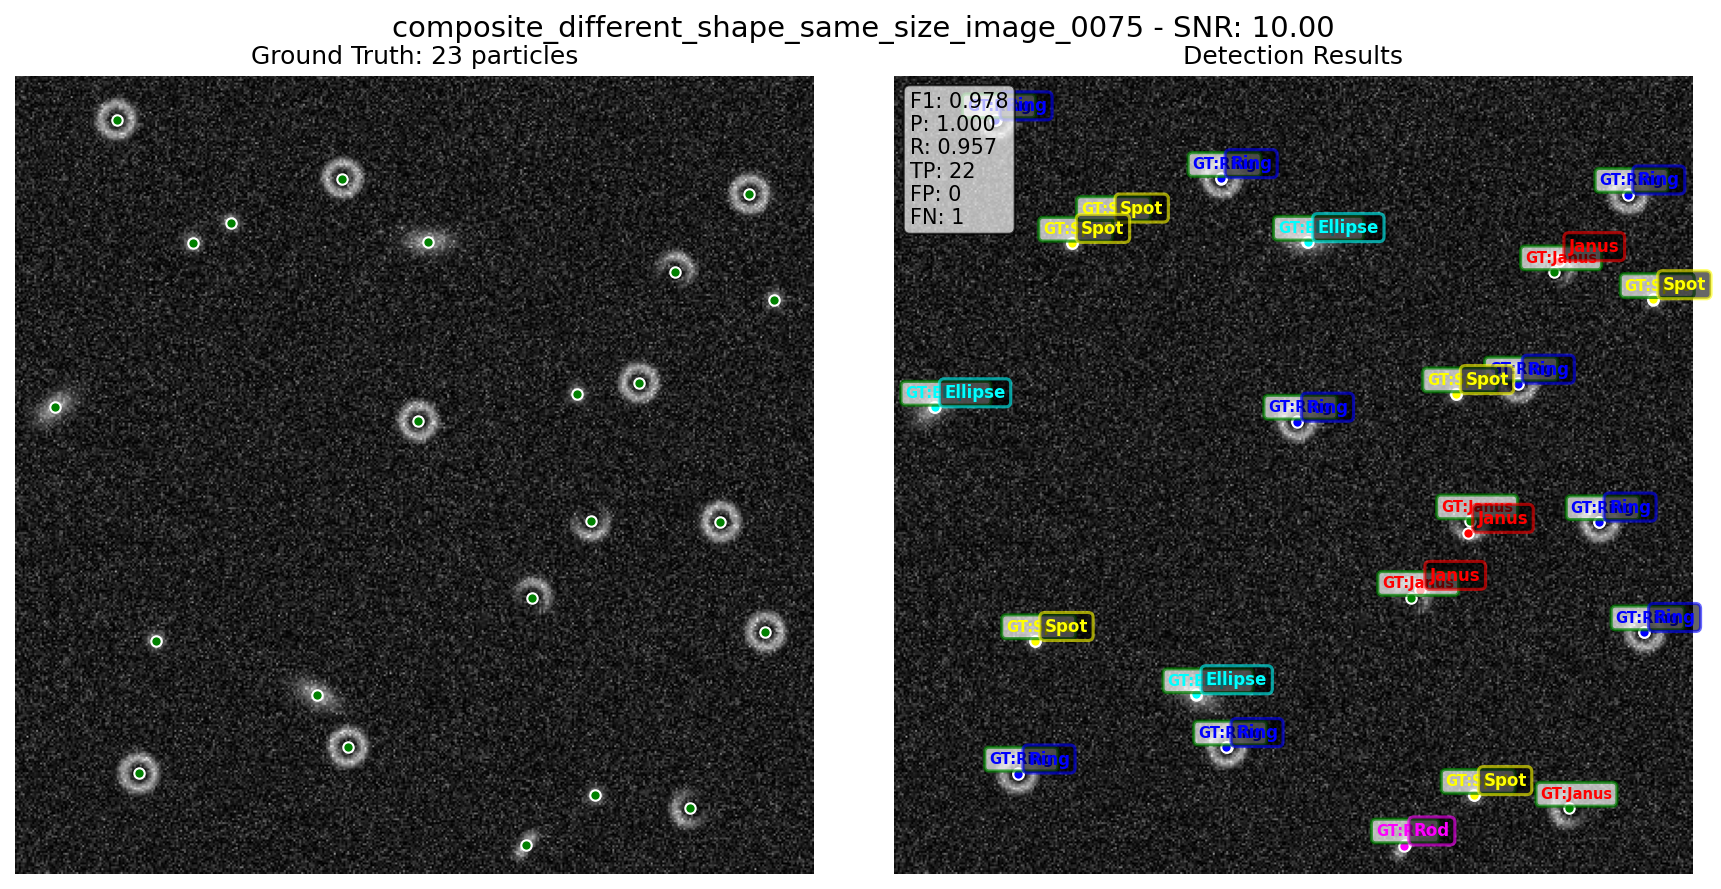
\includegraphics[width=\textwidth]{imglib/Results/composite_different_shape_same_size_image_0075.png}
    \end{figure}
\end{frame}

\begin{frame}{Composite Model Results}
    \begin{figure}
        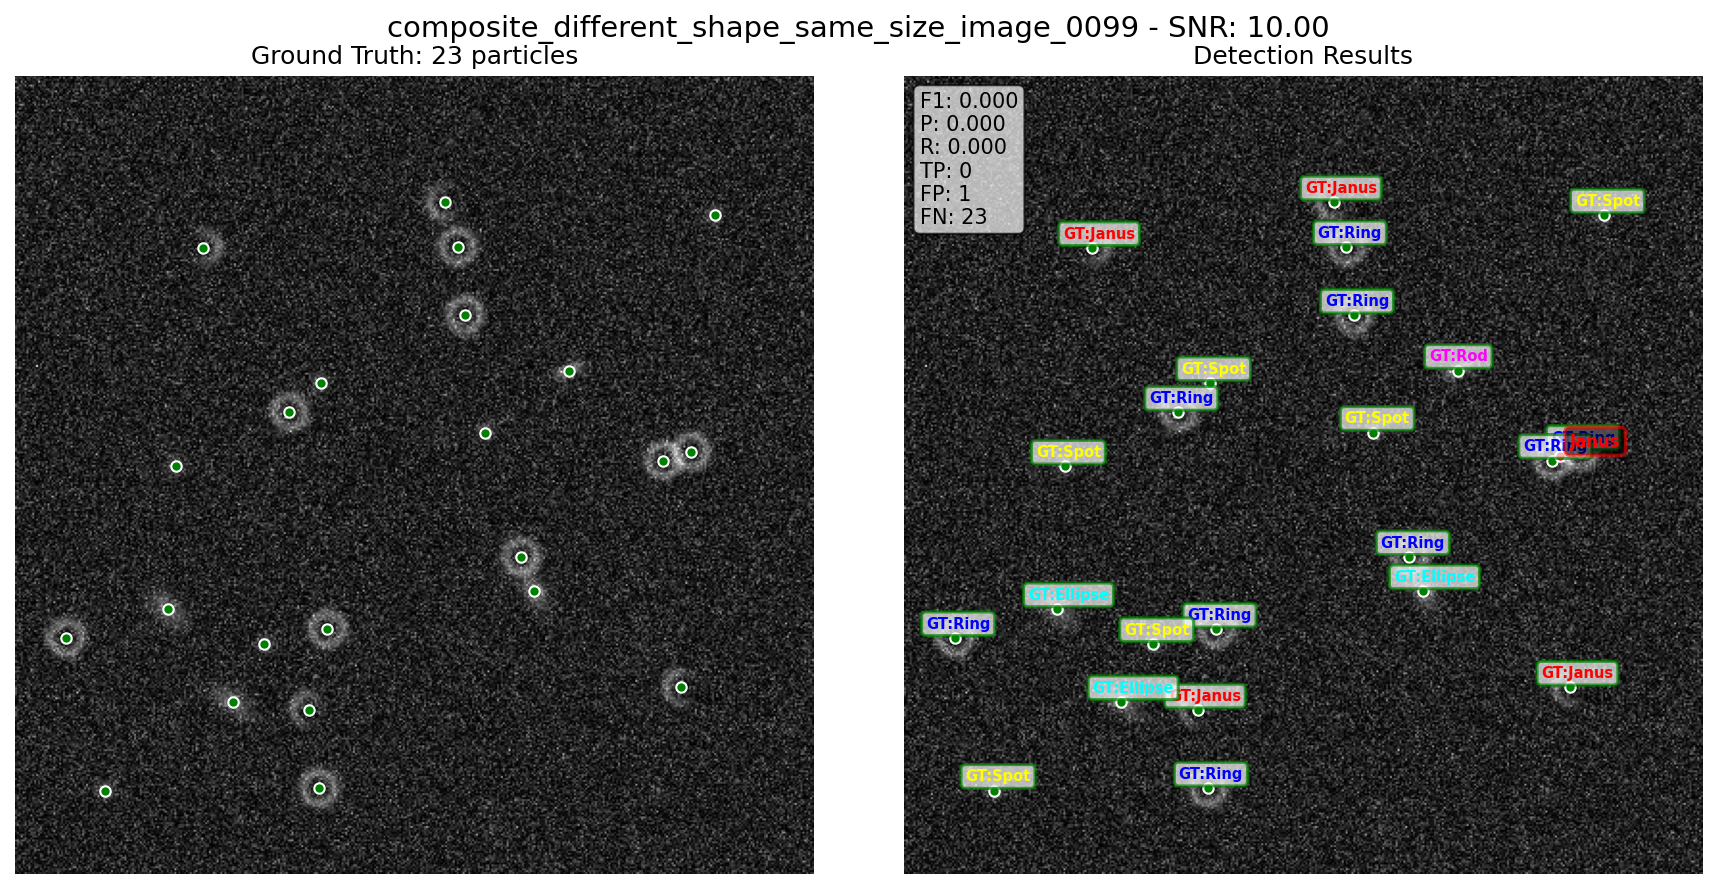
\includegraphics[width=\textwidth]{imglib/Results/composite_different_shape_same_size_image_0099.png}
    \end{figure}
\end{frame}

\begin{frame}{Composite Model Results}
    \begin{figure}
        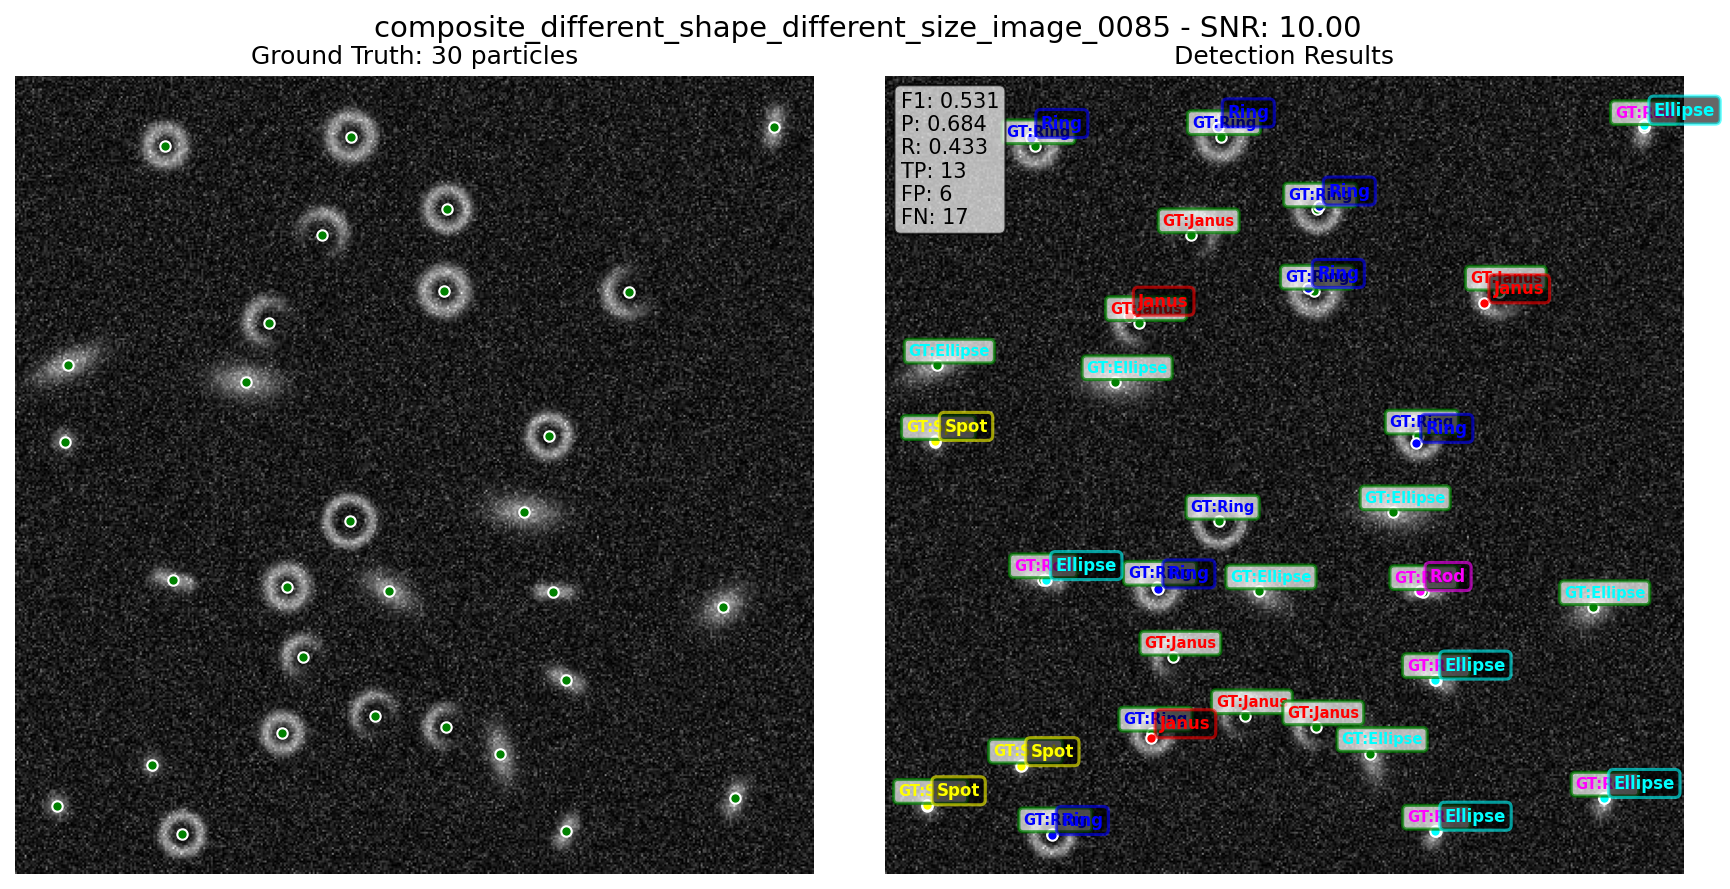
\includegraphics[width=\textwidth]{imglib/Results/composite_different_shape_different_size_image_0085.png}
    \end{figure}
\end{frame}

\begin{frame}{Composite Model Results}
    \begin{figure}
        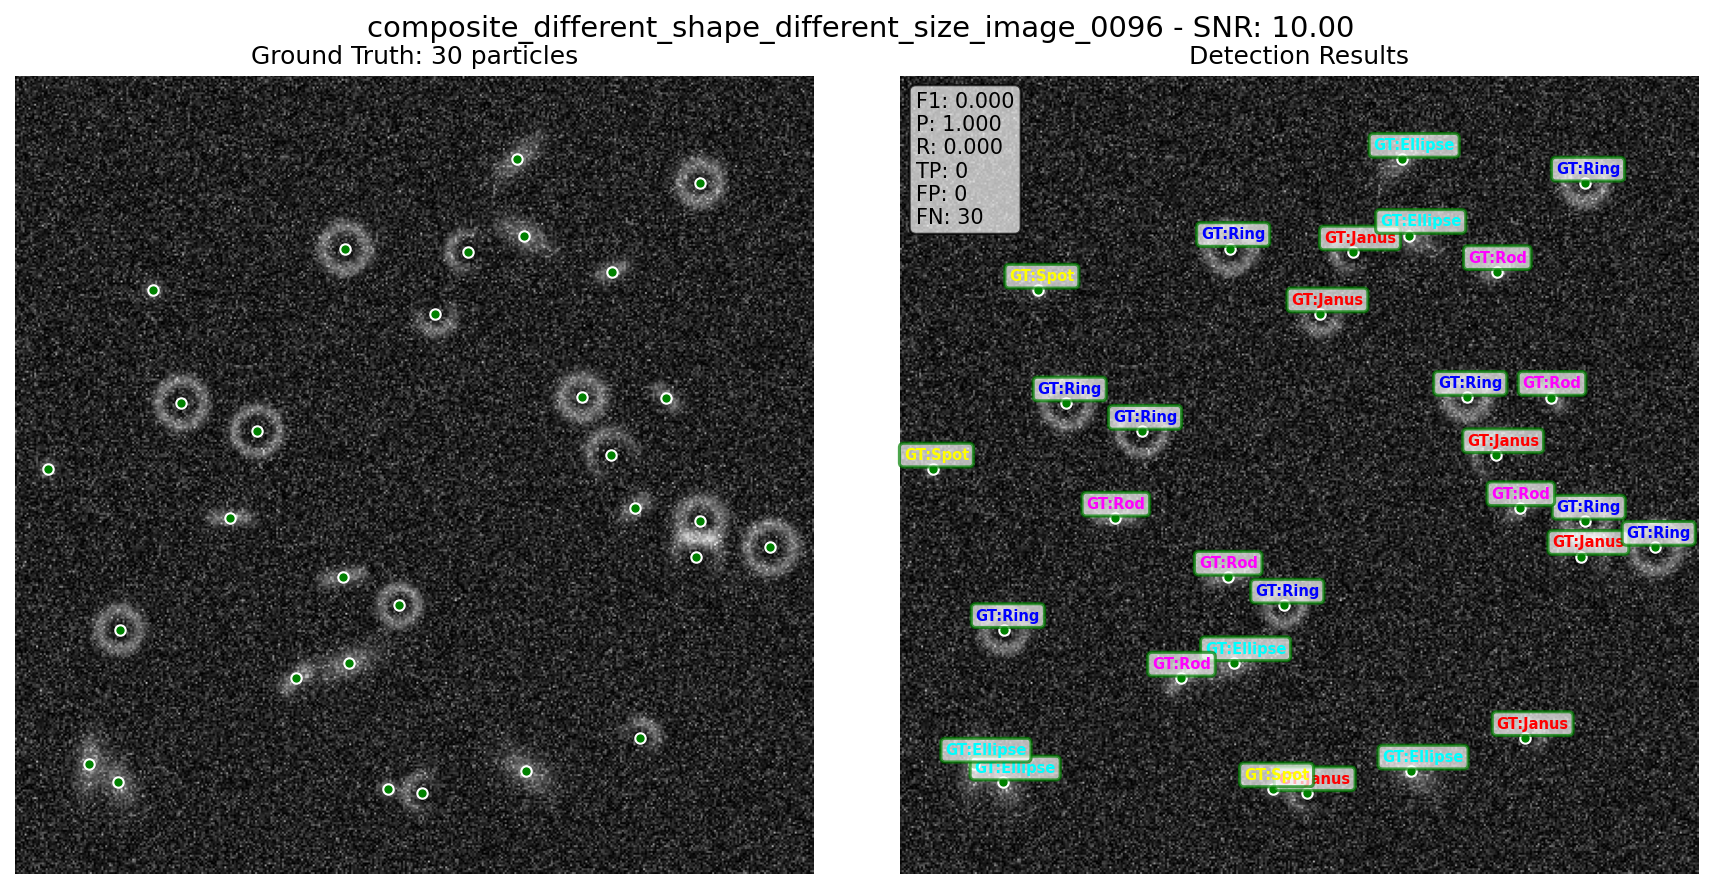
\includegraphics[width=\textwidth]{imglib/Results/composite_different_shape_different_size_image_0096.png}
    \end{figure}
\end{frame}

\begin{frame}{Key Findings \& Future Work}
\begin{columns}
\begin{column}{0.5\textwidth}
\textbf{Key Achievements:}
\begin{itemize}
    \item \textbf{Self-supervised learning} works for particle detection
    \item \textbf{Composite Model} demonstrates high precision and effective classification
    \item \textbf{High recall} on fixed-size scenarios
    \item \textbf{Complete pipeline} implemented successfully
\end{itemize}
\end{column}
\begin{column}{0.5\textwidth}
\textbf{Areas for Improvement:}
\begin{itemize}
    \item \textbf{Scale Invariance}: Add multi-scale training/augmentation to fix low recall on variable sizes
    \item \textbf{Shape-specific training}: Continue optimizing per-particle architectures
    \item \textbf{Complex loss function}: Training with negative samples with modified loss function
    \item \textbf{Custom detection criteria}: Implement custom detection criteria for each particle type
\end{itemize}
\end{column}
\end{columns}
\end{frame}
